\documentclass[twocolumn]{revtex4}
%\documentclass[onecolumn,12pt]{revtex4}
%\usepackage{amsfonts,amssymb,amsmath,mathbbol}              % for math symbols.
%\usepackage{epstopdf}
%\usepackage{mathbbol}              % for math symbols.
\usepackage{graphics,graphicx,epsfig,ulem} 
\usepackage{amsmath}
\usepackage{multirow}
\usepackage{gensymb}
\usepackage{commath}
\usepackage{textcomp}
\newcommand{\squeezeup}{\vspace{-2.5mm}}

\begin{document}

\textheight=26.385cm
%Change textheight as the last resort...

\title{Determining the viscosity of water} 
 
 
\author{Jacky Cao, Room 205, Thursday, Lab Partners: Peter Dorey, Jon Pritchett \\ Date of experiment: 11/11/2016, Date of report: 20/11/2016}


\begin{abstract}              
 
asdkjasnkdnasd

\end{abstract}

\maketitle

\section{Introduction} 
\vspace{-2ex} 

Derived experimentally by Poiseuille in 1838 and Hagen in 1839 \cite{poiseuillehagen}, the volume flow rate $\frac{dV}{dt}$ of a fluid passing through a tube can be expressed as a function of the density of the fluid $\rho$, the value for acceleration due to gravity $g$, the height the fluid leaves the tube $h$, the radius $a$ and length $L$ of the tube, and the viscosity of the fluid $\eta$,

\begin{equation} 
\frac{dV}{dt}=\frac{\pi}{8}\frac{\rho gh}{\eta}\frac{a^4}{L}. 
\label{pohagen}
\end{equation}

Noting that the group $\rho gh$ can be collectively termed the pressure difference $\Delta P$ between the two ends of the tube \cite{collegephysics}.

If we consider that a fluid is flowing through said tube, it experiences both friction with the inner wall and internal friction within itself. The latter can be defined more readily as the viscosity of the fluid $\eta$, and this results in shear stress when two adjacent layers (laminas) of fluid move relative to each other. 

We find that as $\eta$ increases, the volume flow rate decreases, the shear stress between two laminas becomes greater and so restricts the movement of the fluid's molecules trying to flow through the tube. 

Generally we can say that the lamina flow streamlines are smooth, top layers sliding over other laminas without the system having any turbulent motion - this condition is required for equation [\ref{pohagen}] to be valid. 

Using the relation derived by Hagen and Poiseuille it is possible to experimentally calculate a value for the viscosity of water, $\eta_{water}$.

Density of water changes with temperature???!!!

\vspace{-3ex}
\section{Method} 
\vspace{-2ex}
A flow of water was created by fixing a capillary tube to a water tank. The tank was then filled up with water from heights 2cm to 16cm at 2cm intervals, these values were measured with the markings on the side of the tank. During this we had to ensure that we did not create parallax between the level of the water and the markings on the side. 

The water was then allowed to flow out of the tube for a period of 90s for each height of water, this time was measured using a digital stopwatch. As the water flowed out it was caught within a large beaker so that the mass and volume of it could be measured after the allotted time had passed. 

The mass was found by having the beaker already on a set of electronic scales and initially zeroed to account for the beaker's mass. The volume on the other hand required the water to be transferred from the beaker to a measuring cylinder, this was performed by using a pipette. Care was again taken so that there was no parallax and that no unaccounted water was left in the beaker. It was also necessary to clear the tube once air bubbles formed along the length of it, this reduced the flow rate of the water. The bubbles were cleared out using a long piece of copper wire. 

Three total sets of data were taken for each of the three capillary tubes that were used, and with each tube varying in their internal diameter. The first tube had a diameter of 0.110cm, the next at 0.094cm, and the final tube of 0.093cm. These values were calculated from multiple measurements taken using a vernier scale along he horizontal axis, this was repeated to ensure an accurate value could be calculated. 

The collected data was then fitted to a least square fitting to create an initial linear model, then chi-squared analysis was performed to check if the model would hold true and if our data was accurate. 



\begin{figure}[!h]
\begin{center}
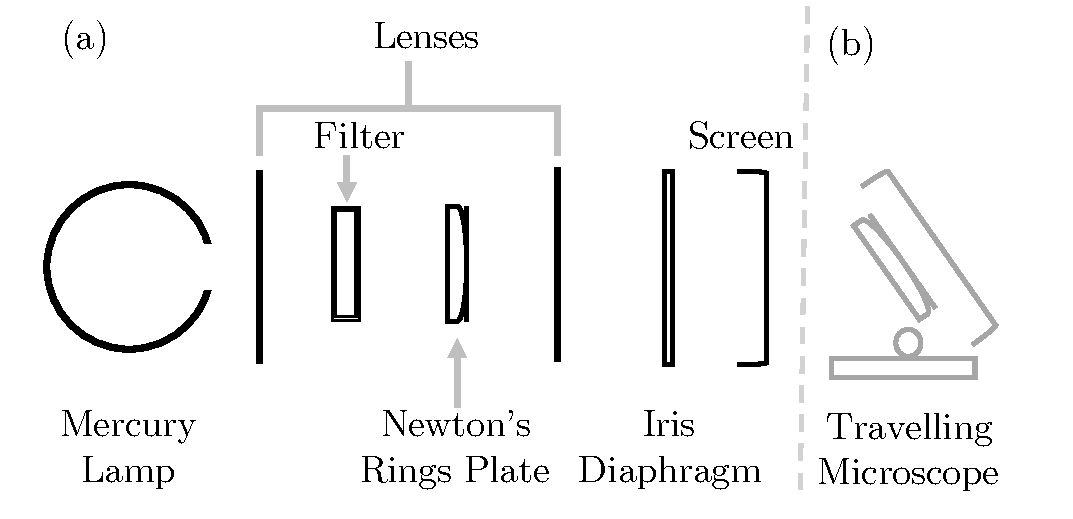
\includegraphics[width=9cm]{fig1}
\caption[]{(a) A schematic of the experimental set-up used to collect the initial set of data. Entire set-up was placed on an optical bench, allowing accurate positioning of the lenses.
\\
(b) Modified set-up used in subsequent investigations - Newton's Rings Plate is moved, the screen is adjusted, and a Travelling Microscope is added.}
\label{fig:fig1}
\end{center}
\end{figure}

askjdnasd

\vspace{-3ex}
\section{Results}
\vspace{-2ex}

asdasd

\vspace{-1ex}
\begin{figure}[!h]
\begin{center}
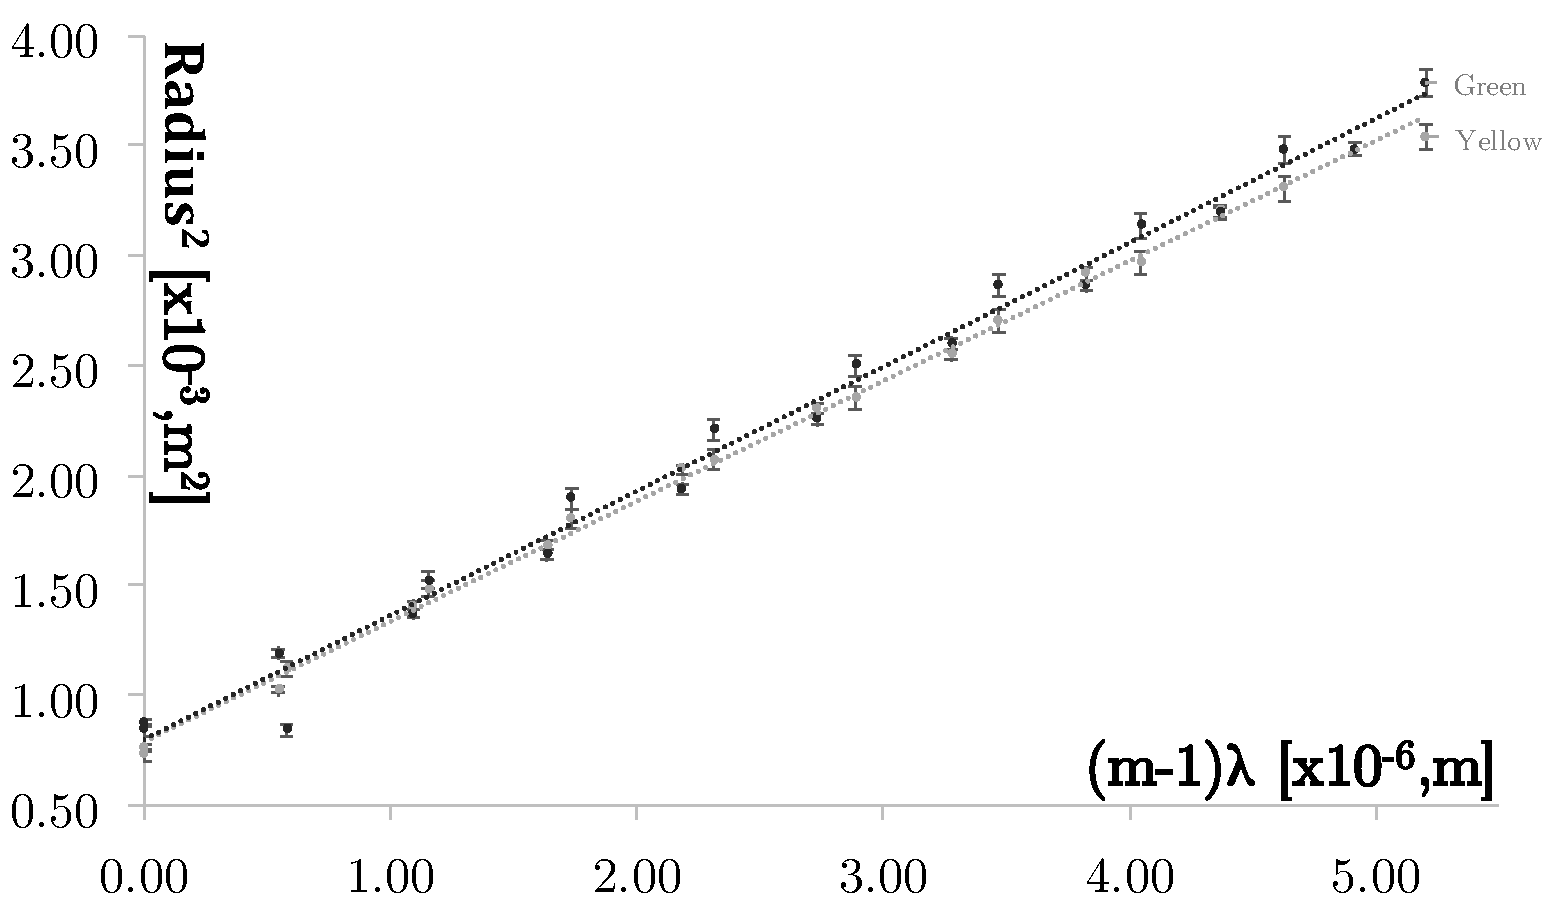
\includegraphics[width=9cm]{fig2}
\caption[]{The fringe radius squared plotted as a function of $(m-1)\lambda$. Horizontal error bars are too small to be seen.}
\label{fig:fig2}
\end{center}
\end{figure}


\begin{table}[h!]
\centering
\begin{tabular}{ |c|c|c|c| } 
 \hline
 \textbf{Tube} & \textbf{Radius, a $[mm]$} & \textbf{$\boldsymbol{\eta_{water}}$ $[mPa]$} & \textbf{$\boldsymbol{\chi^2_v}$}\\ [0.5ex] 
 \hline\hline
 $Blue$ &$0.55\pm0.03$ & $1.5\pm0.4$ & 19.0\\ 
 $Red$ & $0.47\pm0.03$ & $2.5\pm0.7$ & 6.01\\
 $Black$ & $0.46\pm0.03$ & $2.5\pm0.7$ & 27.0\\
 
 \hline
\end{tabular}
\caption{Values for radius of the tube, their respective calculated value for $\eta_{water}$, and the reduced $\chi^2$ value for each value.}
\label{table:1}
\end{table}

\vspace{-3ex}
\section{Discussion}
\vspace{-2ex}

aksdjnkjasndkjnsakjnd


\vspace{-5ex}
\section{Conclusions}
\vspace{-2ex}
 
askjdnjkasd

\begin{thebibliography}{5}
\bibitem{poiseuillehagen}
	Salvatore P. Sutera and Richard Skalak
	\textit{The History of Poiseuille's Law}.
	Annu. Rev. Fluid Mech., 1993.
	
\bibitem{collegephysics}
	Raymond A. Serway, Chris Vuille, and Jerry S. Faughin
	\textit{College Physics, 8th Edition}.
	Brooks/Cole, Belmont, CA, USA, 2009.

\bibitem{youngandfreedman} 
	Hugh D. Young and Roger A. Freedman.
	\textit{University Physics with Modern Physics, 13th Edition}. 
	Pearson Education Limited, Harlow, Essex, 2015.
	
\end{thebibliography}
\clearpage

\vfill
\twocolumngrid
\vspace{-3ex}
\section*{Appendix}
\vspace{-2ex}

The uncertainty calculated for the radius of curvature $R$ was found by propagating other uncertainties related to quantities found in equation (3). The majority of those uncertainties are calculated using equations based off formulae found in \textit{Measurements and their Uncertainties} [I. G. Hughes and T. P. A. Hase, \textit{Measurements and their Uncertainties}, Oxford University Press, Oxford, United Kingdom, 2010]. 
\\

Firstly for the square of the magnified radius of a bright fringe, $\rho_m^2$, the error is, 
\begin{equation} 
\alpha_{r^2}=\alpha_r\abs{2\times r}
\end{equation}

where $r$ is the value for the magnified radius of a bright fringe, and $\alpha_r$ is it's respective uncertainty. In our experiment this value arises due to a 30 cm ruler being used to measure the diameter, so the highest precision achievable would have been limited at half a division, therefore $\alpha_r$=0.5 cm. 

The uncertainty on the magnification squared, $M^2$, is found by,
\begin{equation} 
\alpha_{M^2}=M^2\abs{2\times\frac{\alpha_M}{M}}
\end{equation}

with $\alpha_{M}$ as the error on the magnification. For the initial and repeated experiment this value was taken to be $0.5$ due to the difficulties in measuring the width of one of the tick-marks with a $30$cm ruler. In the Travelling Microscope experiment $\alpha_{M}=0.005$ due to the precision to which we could measure with the vernier scale.    

To calculate the uncertainty on the radius of curvature $R$, the following equation is thus used,
\begin{equation} 
\alpha_R=R\times\sqrt{\Big(\frac{\alpha_n}{n}\Big)^2 + \Big(\frac{\alpha_{M^2}}{M^2}\Big)^2 },
\end{equation}

where the term $n=(m-1)\lambda$, and the uncertainty on that, $\alpha_n$, was found by using a least squares fitting function in the software Microsoft\textregistered \ Excel. $M^2$ is again, the magnification squared with it's uncertainty $\alpha_{M^2}$ found above in equation (5).  

The uncertainty on $d_0$ is found by further propagating the uncertainties found above, the resulting equation is, 

\begin{equation} 
\alpha_{d_0}=d_0\times\sqrt{\Big(\frac{\alpha_c}{c}\Big)^2 + \Big(\frac{\alpha_{M^2}}{M^2}\Big)^2 + \Big(\frac{\alpha_R}{R}\Big)^2}
\end{equation}

where $c$ is the intercept of the least squares fitting, and $\alpha_c$ is it's respective uncertainty.

With the case of the Travelling Microscope there is also the uncertainty on the vernier scale used, we shall take the highest precision it can measure to be $\alpha_{vernier}=0.5$mm.

\clearpage

%\footnotetext{I am not entirely too sure about what I did for (7), it was help from other students and the demonstrator}

\end{document}